%This is a slight variation of the "sig-alternate.tex". We have added a
%\selfcite{myref} command to the sig-alternate.cls file and some explanations to
%the sig-alternate.tex file. Thus, sig-alternate.cls has been renamed to
%dads.cls and sig-alternate.tex has been renamed to dads[nn].tex

% This is "sig-alternate.tex" V1.9 April 2009
% This file should be compiled with V2.4 of "sig-alternate.cls" April 2009
%
% This example file demonstrates the use of the 'sig-alternate.cls'
% V2.4 LaTeX2e document class file. It is for those submitting
% articles to ACM Conference Proceedings WHO DO NOT WISH TO
% STRICTLY ADHERE TO THE SIGS (PUBS-BOARD-ENDORSED) STYLE.
% The 'sig-alternate.cls' file will produce a similar-looking,
% albeit, 'tighter' paper resulting in, invariably, fewer pages.
%
% ----------------------------------------------------------------------------------------------------------------
% This .tex file (and associated .cls V2.4) produces:
%       1) The Permission Statement
%       2) The Conference (location) Info information
%       3) The Copyright Line with ACM data
%       4) NO page numbers
%
% as against the acm_proc_article-sp.cls file which
% DOES NOT produce 1) thru' 3) above.
%
% Using 'sig-alternate.cls' you have control, however, from within
% the source .tex file, over both the CopyrightYear
% (defaulted to 200X) and the ACM Copyright Data
% (defaulted to X-XXXXX-XX-X/XX/XX).
% e.g.
% \CopyrightYear{2007} will cause 2007 to appear in the copyright line.
% \crdata{0-12345-67-8/90/12} will cause 0-12345-67-8/90/12 to appear in the copyright line.
%
% ---------------------------------------------------------------------------------------------------------------
% This .tex source is an example which *does* use
% the .bib file (from which the .bbl file % is produced).
% REMEMBER HOWEVER: After having produced the .bbl file,
% and prior to final submission, you *NEED* to 'insert'
% your .bbl file into your source .tex file so as to provide
% ONE 'self-contained' source file.
%
% ================= IF YOU HAVE QUESTIONS =======================
% Questions regarding the SIGS styles, SIGS policies and
% procedures, Conferences etc. should be sent to
% Adrienne Griscti (griscti@acm.org)
%
% Technical questions _only_ to
% Gerald Murray (murray@hq.acm.org)
% ===============================================================
%
% For tracking purposes - this is V1.9 - April 2009

\documentclass{dads}   %Changed for DADS

\usepackage{algpseudocode}
\usepackage{algorithm}
\usepackage{amsmath}
\usepackage{amssymb}

\begin{document}
% --- Author Metadata here ---
\conferenceinfo{SAC'19}{April 8--12, 2019, Limassol, Cyprus}
\CopyrightYear{2019} % Allows default copyright year (200x) to be over-ridden - IF NEED BE.
%\crdata{0-12345-67-8/90/01}  % Allows default copyright data (0-89791-88-6/97/05) to be over-ridden - IF NEED BE.
% --- End of Author Metadata ---

\title{Alternate {\ttlit ACM} SIG Proceedings Paper in LaTeX
Format\titlenote{(Produces the permission block, and
copyright information). For use with
SIG-ALTERNATE.CLS. Supported by ACM.}}

\subtitle{[Slightly extended for DADS]
\titlenote{A full version of this paper is available as
\textit{Author's Guide to Preparing ACM SIG Proceedings Using
\LaTeX$2_\epsilon$\ and BibTeX} at
\texttt{www.acm.org/eaddress.htm}}}
%
% You need the command \numberofauthors to handle the 'placement
% and alignment' of the authors beneath the title.
%
% For aesthetic reasons, we recommend 'three authors at a time'
% i.e. three 'name/affiliation blocks' be placed beneath the title.
%
% NOTE: You are NOT restricted in how many 'rows' of
% "name/affiliations" may appear. We just ask that you restrict
% the number of 'columns' to three.
%
% Because of the available 'opening page real-estate'
% we ask you to refrain from putting more than six authors
% (two rows with three columns) beneath the article title.
% More than six makes the first-page appear very cluttered indeed.
%
% Use the \alignauthor commands to handle the names
% and affiliations for an 'aesthetic maximum' of six authors.
% Add names, affiliations, addresses for
% the seventh etc. author(s) as the argument for the
% \additionalauthors command.
% These 'additional authors' will be output/set for you
% without further effort on your part as the last section in
% the body of your article BEFORE References or any Appendices.

\numberofauthors{1} %  in this sample file, there are a *total*
% of EIGHT authors. SIX appear on the 'first-page' (for formatting
% reasons) and the remaining two appear in the \additionalauthors section.
%
\author{
% You can go ahead and credit any number of authors here,
% e.g. one 'row of three' or two rows (consisting of one row of three
% and a second row of one, two or three).
%
% The command \alignauthor (no curly braces needed) should
% precede each author name, affiliation/snail-mail address and
% e-mail address. Additionally, tag each line of
% affiliation/address with \affaddr, and tag the
% e-mail address with \email.
%
\alignauthor
No author info because of double-blind review.
% 1st. author
%\alignauthor
%Ben Trovato\titlenote{Dr.~Trovato insisted his name be first.}\\
%       \affaddr{Institute for Clarity in Documentation}\\
%       \affaddr{1932 Wallamaloo Lane}\\
%       \affaddr{Wallamaloo, New Zealand}\\
%       \email{trovato@corporation.com}
%% 2nd. author
%\alignauthor
%G.K.M. Tobin\titlenote{The secretary disavows
%any knowledge of this author's actions.}\\
%       \affaddr{Institute for Clarity in Documentation}\\
%       \affaddr{P.O. Box 1212}\\
%       \affaddr{Dublin, Ohio 43017-6221}\\
%       \email{webmaster@marysville-ohio.com}
%% 3rd. author
%\alignauthor Lars Th{\o}rv{\"a}ld\titlenote{This author is the
%one who did all the really hard work.}\\
%       \affaddr{The Th{\o}rv{\"a}ld Group}\\
%       \affaddr{1 Th{\o}rv{\"a}ld Circle}\\
%       \affaddr{Hekla, Iceland}\\
%       \email{larst@affiliation.org}
%\and  % use '\and' if you need 'another row' of author names
%% 4th. author
%\alignauthor Lawrence P. Leipuner\\
%       \affaddr{Brookhaven Laboratories}\\
%       \affaddr{Brookhaven National Lab}\\
%       \affaddr{P.O. Box 5000}\\
%       \email{lleipuner@researchlabs.org}
%% 5th. author
%\alignauthor Sean Fogarty\\
%       \affaddr{NASA Ames Research Center}\\
%       \affaddr{Moffett Field}\\
%       \affaddr{California 94035}\\
%       \email{fogartys@amesres.org}
%% 6th. author
%\alignauthor Charles Palmer\\
%       \affaddr{Palmer Research Laboratories}\\
%       \affaddr{8600 Datapoint Drive}\\
%       \affaddr{San Antonio, Texas 78229}\\
%       \email{cpalmer@prl.com}
}
%% There's nothing stopping you putting the seventh, eighth, etc.
%% author on the opening page (as the 'third row') but we ask,
%% for aesthetic reasons that you place these 'additional authors'
%% in the \additional authors block, viz.
%\additionalauthors{Additional authors: John Smith (The Th{\o}rv{\"a}ld Group,
%email: {\texttt{jsmith@affiliation.org}}) and Julius P.~Kumquat
%(The Kumquat Consortium, email: {\texttt{jpkumquat@consortium.net}}).}
\date{30 July 1999}
% Just remember to make sure that the TOTAL number of authors
% is the number that will appear on the first page PLUS the
% number that will appear in the \additionalauthors section.

\maketitle
\begin{abstract}
This paper provides a sample of a \LaTeX\ document which conforms,
somewhat loosely, to the formatting guidelines for
ACM SIG Proceedings. It is an {\em alternate} style which produces
a {\em tighter-looking} paper and was designed in response to
concerns expressed, by authors, over page-budgets.
It complements the document \textit{Author's (Alternate) Guide to
Preparing ACM SIG Proceedings Using \LaTeX$2_\epsilon$\ and Bib\TeX}.
This source file has been written with the intention of being
compiled under \LaTeX$2_\epsilon$\ and BibTeX.

The developers have tried to include every imaginable sort
of ``bells and whistles", such as a subtitle, footnotes on
title, subtitle and authors, as well as in the text, and
every optional component (e.g. Acknowledgments, Additional
Authors, Appendices), not to mention examples of
equations, theorems, tables and figures.

To make best use of this sample document, run it through \LaTeX\
and BibTeX, and compare this source code with the printed
output produced by the dvi file. A compiled PDF version
is available on the web page to help you with the
`look and feel'.
\end{abstract}

% A category with the (minimum) three required fields
\category{H.4}{Information Systems Applications}{Miscellaneous}
%A category including the fourth, optional field follows...
\category{D.2.8}{Software Engineering}{Metrics}[complexity measures, performance measures]

\terms{Delphi theory}

\keywords{ACM proceedings, \LaTeX, text tagging}

\section{Introduction}
All cryptocurrencies, in particular, Bitcoin (the worlds most used cryptocurrency) maintain a decentralized record that keeps track of all transactions that have happened in a chronological order~\cite{nakamoto2008bitcoin}. The ability to maintain a decentralized record that can be updated by almost anyone has attracted the attention of a lot of other fields beyond the cryptocurrency market where this concept was introduced. For instance, a distributed record could be used to keep a record of transactions, contracts and all other kinds of information that, if we wanted to save them, we would have to speak with a notary. \footnote{For a list of examples, refer to \url{https://blockgeeks.com/guides/blockchain-applications/}}

This distributed record is usually maintained in the following manner.  Firstly, for efficiency reasons, multiple transactions are grouped together, this groups of transactions are called a\textit{blocks}. Afterwards, blocks are linked between them to form a linked list which is called \textit{blockchain}. This linked list enforces a chronological order over the blocks and as a consequence over the transactions inside the blocks. An interesting aspect of cryptocurrencies, like Bitcoin, is that they use a decentralized open peer-to-peer membership system. This means that nodes do not have to know all the other nodes of the system, and any node can join or leave the network at any given time that the protocol assures consistency of the record even if a few nodes might have a rational or byzantine behaviour.

Usually, the system that maintains the blockchain works in the following manner. The nodes of the system, concurrently, receive transactions, validate them and relay them to other nodes. Furthermore, each node attempts to generate the next block in the chain, to do this they try to solve a challenging cryptographic puzzle called proof of work. When a node finally generates a block, it will broadcast it through the network which will make all other nodes cancel the generation of concurrent blocks to the one being broadcast and start trying to generate a new block. Before accepting and relaying a block, each node validates the blocks it receives.

By the brief description above, it easy to realise that the relay of transactions is a core process for any distributed ledger. Firstly, the transactions need to reach the nodes that are generating blocks so that they can be added to a block. Secondly, they also need to reach other nodes allowing them to validate blocks. In Bitcoin, the broadcast of transactions works by nodes periodically advertising to their neighbours the transactions that they have. Their neighbours upon, receiving the advertisements for transactions that they still do not have, will send requests for those transactions to the nodes who sent the advertise. This process generates a redundancy of advertising messages. However, despite this redundancy begin desirable allowing the system to cope with failures, we found out that each node receives an excessive amount of duplicated advertisements for each transaction.

In this article, we propose a modification in the transaction broadcasting system of \textit{Bitcoin} that improves its efficiency. Our adjustments take advantage of already existing asymmetries in the network. In fact, in a \textit{Bitcoin} network only a fraction of the network, about 10\%, spends resources generating new blocks without being associated with a mining pool (these nodes are called miners), the majority of nodes just relay information and maintain a copy of the blockchain. Our strategy consists in skewing the broadcasting of transactions so that they reach miners faster and at the same time lowering the amount of duplicated advertisements. This strategy takes advantage of, not only the weak latency requirements around the broadcasting transactions in Bitcoin between non-miners nodes, but also takes advantage of messages types introduced in the previous year, that allow for a much more efficient dissemination of transactions once they are added to a block. An experimental evaluation of the changes proposed show a reduction in 10.7\% of the bandwidth consumed and a reduction of 40.5\% in the total number of messages exchanged, without any negative impact in the resilience of the system.

\section{The {\secit Bitcoin} ledger}
Bitcoin was created back in 2009 with the main objective of providing a system where two entities can exchange goods in a secure and anonymous way without having to trust each other or any third entity. To achieve this goal the system uses a crypto coin, that can be exchanged between the parties involved in a transaction. All the transactions are grouped in blocks and registered in the distributed ledger. Furthermore, the ledger keeps track of all the coins that have been spent, which forbids users from trying to spend the same coin twice (attacks that try to defeat this system are entitled as \textit{double spending} attacks). The Bitcoin ledger is built by linking each block to its predecessor hence forming an infinite chain of block named \textit{blockchain}.

The protocol to maintain the Bitcoin ledger is quite complex with many moving parts and functionalities that complement each other. Firstly, Bitcoin has membership algorithms that try to ensure that each node maintains connections to other nodes of the systems chosen randomly. This connections between the nodes form an overlay that is then used to disseminate information, namely: the transactions created by clients and the blocks generated.

As referred previously, new blocks are generated concurrently by nodes named miners. Each miner picks a group of transactions to form a block. For a block to be considered valid, not only has to contain only valid transactions inside but also, has to contain a proof that the node solved the cryptographic puzzle. This cryptographic puzzle is influenced mainly by the content inside the block like the hash of the previous block and the transactions inside the new block. This has two advantages. First, it disincentivizes the creation of blocks with invalid transactions inside it, because the only way a node get recompensated by creating a block is if his block gets accepted into the blockchain. Furthermore, the difficulty of the puzzle lowers the probability of two nodes generating a block at the same time, which if it happens would generate a fork in the chain. Note that as transactions take different times to reach different nodes, it is certain that the group of transactions chosen by two nodes to add to their blocks will be different. Hence, this will result in two different crypto puzzles for each node to solve. When a new block is generated it is broadcast through the network. To avoid corrupted or invalid blocks from being broadcast, each node has to validate a block before broadcasting it. For a block to be considered valid it has to has the following information: hash of the previous block and all the transactions inside it (to be able to validate the transactions). A transaction is valid when it does not try to spend an already spent coin. If a node does not have all these pieces of information it has to wait before relaying the block.

If a node receives a block at the same height as the one he is trying to mine, the process of mining is interrupted. This behaviour also lowers the probability of two different blocks at the same height begin generated at the same time. However, in the case, they are and are broadcast through the network a fork will happen in the chain and to solve this fork the network will then adopt the branch which is higher. This is done by nodes aborting the mining process when they realise they are working on a smaller branch and start trying to mine on the higher branch.

The algorithms used by Bitcoin to disseminate transactions and blocks have evolved over the years and recently introduced mechanisms to prevent wasting bandwidth. We are now going to go over a simple overview of the protocol. As referred previously, transactions are broadcast through advertisements sent in \textsl{Inv} messages that contain the set of transactions known by the sender. When a node receives a \textsl{Inv} message it determines which transactions it does not possess and sends a \textsl{GetData} message requesting those transactions. Finally, when a node receives a \textsl{GetData} it will reply with a \textsl{TX} message for each transaction requested. Regarding blocks, blocks are disseminated mainly in two ways. The first one and older is through advertisements similar to transactions. Once a block is found is sent a \textsl{Headers} message advertising the block. When a node receives a \textsl{Headers} message containing the header of a new block it will request it using a \textsl{GetData} message and will then receive a block through a \textsl{Block} message. The second strategy for broadcasting blocks consists in sending a summary o the block through the  \textsl{CmpctBlock} (compact block) message. When validating a block after having received it by a \textsl{CmpctBlock} message if the node does not possess all the transactions to validate the block it can send a \textsl{GetBlockTX} requesting them. The first strategy has as an advantage the fact that the nodes do not need to exchange more message between them but as a disadvantage, it generates more redundancy since all the transactions are sent with the block and there is a high probability that the node already has all transactions needed to validate the block.

Additionally, each node maintains or each neighbour a queue that containing messages to be sent in the future. When a new \textsl{TX} is received, after being validated is added to the queue of each neighbour. These queues are updated every time a \textsl{TX} or a \textsl{Block} is received to prevent the nodes from sending information that a node already has. Periodically these queues are flushed and the node sends the \textsl{Inv} messages to the respective neighbours containing the content of the queue of each one.

Although there are already some attempts to lower the amount of bandwidth consumed and the number of messages sent this system still possesses some inefficiencies discussed in the next section.

\section{Improvement in the broadcast of transactions}
In this section, we propose a set of changes to the dissemination algorithm of transactions with the objective of making it more efficient, namely by lowering the number of redundant advertisements that each node receives. Our proposal is based on the following observations:

\begin{itemize}
  \item Currently, each node receives on average $6.6$ duplicated advertisements for each transaction (when would be enough receiving a single one to ensure the reception of a transaction).
  \item The network currently possesses two procedures to disseminate transactions: exhange of advertisements (used when a transaction is not in a block) exchange of block (used when a transaction is already added to a block).
  \item For historical reasons, the second mechanism is more efficient than the first one, because all missing transactions a node might request are sent in a single message (meanwhile through the advertisement method a node has to send a message for each individual transaction).
  \item In Bitcoin, the constraints for the broadcasting of transactions are weak because the rate of generation of the blocks is much slower than the processes of dissemination of transactions (on average a block is generated once every 10 minutes)
  \item Miners are only a small fraction of the total number of nodes in the network. And although it essential that transactions reach miners the protocol does not distinguish miners from the rest of the nodes.
  \item In the current protocol, nodes send their advertisements to all their neighbours (125 in the worst case). This value is substantially higher than the theoretical value for epidemic broadcasting algorithms, which suggests that even in the presence of failures its enough to send information for a number of neighbours proportional to the size of the network which is approximately around 10 000 nodes hence it would be enough to send to $ ln(10~000) \approx 10$ neighbours.
\end{itemize}

The main objective is to lower the amount of duplicated advertisements in the network and at the same time ensure that the transactions reach the miners. The intuition for the proposed approach is to skew the process of dissemination in the direction of the most productive miners. Without however putting the resilience of the system at stake by broadcasting the information to the rest of the system through alternative paths. This is achieved through tree changes to the protocol. The first modification consists in saving for each block that we receive from a neighbour the time that neighbour took to disseminate the block to us. The second one is also for each neighbour maintain a list with the transactions we sent to him a how much time it took for those transactions to be added to a block. Finally, the third change is locally determining which path is better for sending our transactions so that they reach the miners faster and give priority to these paths in the dissemination process. Note that once a transaction is added to a block the epidemic dissemination process becomes irrelevant.

\subsection{Ranking neighbours}
As referred previously, the strategy proposed to lower the bandwidth used, has a requirement that each node discovers which path is the fastest to reach the miners. The miners to where we have the fastest paths will rank higher in the list, and the ones with the slowest paths will rank at the bottom of the list.

To obtain this ranking of the neighbours each node will have to maintain for each neighbour five variables:
\begin{itemize}
  \item \textit{n} total number of blocks received by that neighbour;
  \item \textit{k} accumulated time it took to disseminate a block to us;
  \item \textit{a} total number of blocks received;
  \item \textit{z} total number of transactions we sent to that neighbour;
  \item \textit{y} accumulated time it took for those transactions to be accepted in a block.
\end{itemize}

The time it takes for a neighbour to relay a block until a node is given by the difference between the current time and the last time the node received a new block from that neighbour. If a neighbour takes more than four hours to relay a block to a node the difference will be the current time minus four hours.  If Given the large number of transactions that flow through the network, instead of maintaining timers for all of them we only maintain a timer each one hundred transactions. This way we do not overburden nodes with metadata.

\begin{displaymath} \mbox{class}^{T}= (\dfrac{k^{T}}{n^{T}} + a^{T} - n^{T} + \dfrac{y^{T}}{z^{T}}) \end{displaymath}

With this classification, we prevent nodes that only generate a block once in a while from having a good classification eternally.

This is important because as we have said, there is still a percentage of blocks being mined by random nodes, and if we would, for instance, send all our transactions to those nodes they would take a lot of time to appear in a block. Which is not desired, given that the average time it takes for a transaction to be accepted in Bitcoin nowadays is ten minutes.

This way for a neighbour to have good classification it has to have a good ratio of time it takes to disseminate blocks/number of blocks we received from him, a good ratio of blocks received from him/blocks received and finally a good ratio of time it took for a transaction to be added to blocks if we sent it to him.

Give that the classification of neighbours is prone to change over time, the actual value used to order neighbours is given by the following sliding average of the classification presented previously:

\begin{displaymath} \mbox{class}^t = (1-\alpha) \cdot \mbox{class}^{t-1} + \alpha \cdot \mbox{class}^{T} \end{displaymath}

The $\alpha$ factor exists to avoid nodes that once generated a lot of blocks but currently do not from having a good classification forever. In our experiments, we used an $\alpha=0.3$ and a \textit{T} configured to be an interval of four hours.

Each time a node receives a block from a neighbour the classification of the neighbours will be updated using Algorithm~\ref{alg:class}

\begin{algorithm}[t]
\begin{algorithmic}[1]
\Function{update\_nodes\_classification}{\textsl{node\_to\_update}}
\State $\textsl{scores} \gets \textsl{[ ]}$
\For{$node$ \textbf{in} $neighbourhood$}
  \State $\textsl{score} \gets \textsl{get\_classification(node)}$
  \State $\textsl{scores.append([score, id])}$
\EndFor
\State $sort(\textsl{scores})$
\State $\textsl{top\_nodes} \gets \textsl{[ ]}$
\For{$i$ \textbf{in} $range(0, max\_top\_nodes)$}
  \State $\textsl{top\_nodes.append(score[i][1])}$
\EndFor
\EndFunction
\end{algorithmic}
\caption{Top neighbours computation}
\label{alg:class}
\end{algorithm}

\subsection{Skewed relay}
\label{sec:sr}
Given that our objective is that our transactions reach a miner as fast as possible we can use the mechanism described previously to do it. Hence, if all the nodes were to follow the protocol correctly, and the paths created by out solution were resilient enough we could send our transactions to only one node, and they would eventually appear in a block.

However, even if we do not consider the problem of nodes disconnecting from the network, there is the problem of time it takes for a transaction to be committed. So to solve this problem, we will send our transactions not only to the \textit{t} top nodes but also to \textit{r} random nodes, as it is described in Algorithm~\ref{alg:diss}. This way we assure that our transactions are still broadcast through the rest of the network and will be committed in a timely manner.

\begin{algorithm}[t]
\begin{algorithmic}[1]
\Function{nodes\_to\_send}{tx}
\If{$(ip == True$ \textbf{and} $tx.source() == self)$}
	\State {$\textbf{return}$ $neighbours$}
\EndIf
\State $\textsl{total} \gets \textsl{max\_t\_nodes} + \textsl{max\_r\_nodes}$
\If{$size(neighbours) < total$}
	\State $\textsl{total} \gets \textsl{size(neighbours)} - \textsl{max\_t\_nodes}$
\Else
	\State $\textsl{total} \gets \textsl{total} - \textsl{max\_t\_nodes}$
    \EndIf
\If{$total > 0$}
	\State $\textsl{r\_nodes} \gets \textsl{rand\_choice(neighbours, max\_r\_nodes)}$
    \EndIf
\State \Return t\_nodes + r\_nodes
\EndFunction
\end{algorithmic}
\caption{Nodes to send transactions advertisements computation}
\label{alg:diss}
\end{algorithm}

The value of Initial Push (ip) indicates that if a transaction is generated by a node, the node has the option of either sending it for only \textit{t} plus \textit{r} or to all his neighbours.

Hence we can then configure the following variables \textsl{ax\_top\_nodes}, \textsl{max\_top\_nodes} and \textsl{ip} to obtain different results in the information dissemination. In Chapter~\ref{sec:evaluation} we will dicuss diferent configurations tested.

\subsection{Complying with network changes}
A key aspect of peer-to-peer networks as stated previously is that nodes can leave or join the network at any given time. With this in mind and also the fact that is not possible to exactly determine which node is going to mine the next block, we designed an algorithm that adapts to the network in order to maintain the commit time of the transactions while still trying to send as few messages as possible. Our algorithm increases or decreases the values of \textsl{max\_t\_nodes} and \textsl{max\_r\_nodes} by one depending if either, our transactions are taking too long to be committed to a bock or if they are being committed in a reasonable time as depicted in Algorithm~\ref{alg:inc}.

\begin{algorithm}[t]
\begin{algorithmic}[1]
\Function{increase\_relay}{}
\State $\textsl{avg\_time} \gets \textsl{get\_avg\_time\_unconfirmed()}$
\State $\textsl{timeout} \gets \textsl{avg\_time() > TIME\_TX\_CONFIRM}$
\State $\textsl{space} \gets \textsl{max\_t\_nodes + 1 <= neighbourhood / 2}$
\State $\textsl{cooldown} \gets \textsl{time\_since\_last\_inc + TIME\_TO\_WAIT <= now}$
\If{$timeout$ \textbf{and} $space$ \textbf{and} $cooldown$}
  \State $increase(t, r, 1)$
  \State $\textsl{had\_to\_inc} \gets \textsl{True}$
  \State $update\_nodes\_classification()$
  \State $time\_since\_last\_inc = now$
  \State $relay\_delayed\_TX()$
\EndIf
\State $\textsl{cooldown} \gets \textsl{time\_since\_last\_dec + TIME\_TO\_WAIT <= now}$
\If{\textbf{not} $had\_to\_inc$ \textbf{and} $cooldown$}
  \State $\textsl{avg\_time} \gets \textsl{get\_avg\_time\_confirmed()}$
  \State $\textsl{timeout} \gets \textsl{avg\_time() <= TIME\_TX\_CONFIRM}$
  \State $\textsl{space} \gets \textsl{max\_t\_nodes - 1 <= 0}$
  \If{$timeout$ \textbf{and} $space$}
    \State $decrease(t, r, 1)$
    \State $update\_nodes\_classification()$
    \State $time\_since\_last\_dec = now$
  \EndIf
\EndIf
\EndFunction
\end{algorithmic}
\caption{Increase or decrease top and random lists computation}
\label{alg:inc}
\end{algorithm}

As shown in Algorithm~\ref{alg:inc} if the current average, of the time it takes for the unconfirmed transactions of a node to be committed to a block, gets bigger than the constant \textsl{TIME\_TX\_CONFIRM} (30 minutes) then the node is going to increase both the size of \textsl{max\_t\_nodes} and \textsl{max\_r\_nodes}, relay the transactions that took more than 30 minutes to commit. If for instance, all the current average of the unconfirmed transactions does not surpass the threshold of the 30 minutes then, the node will check if the average time it took to confirm its transactions confirmed in the last hour took less than \textsl{TIME\_TX\_CONFIRM} if yes then the node will reduce \textsl{max\_t\_nodes} and \textsl{max\_r\_nodes} by one else it will not do anything. Each time \textsl{max\_t\_nodes} and \textsl{max\_r\_nodes} are changed the node will not be able to change these values in the next 2 hours to prevent fluctuations in these values. Furthermore, every time a node increases \textsl{max\_t\_nodes} and \textsl{max\_r\_nodes} it will not be able to decrease these values in the next 4 hours in order to preserve resilience over performance.

\section{Evaluation}
To evaluate the proposed approach, we built an event simulator that modules the broadcast of transactions and blocks in the Bitcoin network (this simulator was developed in python). We decided to implement our own simulator because all the simulators that we found were either outdated or were not working.

\subsection{Simulator tunnig}
In order to tune our simulator so that it simulates the original protocol faithfully, we extended the \textsl{Bitcoin Core} client, the most used Bitcoin client to log metrics about the messages exchanged between clients. The metrics logged were the folowing: i) transactions advertisements; ii) received transactions; iii) transactions present in compact blocks that the node had to request to be able to rebuild the block. We deployed two instances of this client in two distinct physical locations for a whole month and used the metrics logged by these two clients to tune our simulator. Furthermore, we also used information publicly available on the website \url{https://blockchain.info/} to determine the number of transaction generated, the distribution of blocks generated by miners and the average transaction size. With all these metrics we implemented the original protocol, and then we added our changes to the protocol. We experimentally tunned our simulator so that the results observed were the same as the ones observed in the real client. The network model that we used in our simulations was composed solely of nodes that followed the protocol accordingly.

Running simulations of big Bitcoin networks in a language not optimized for efficiency resulted in the simulations being very demanding in terms of computations and space required which resulted in the simulations taking a long time (scale of days) to complete. Because of this, we tried to see if lowering the size of the network was going to impact the results. To do this we ran the original protocol with 6000 nodes and with 625 nodes and compared the metrics discussed further. The results we obtained were equivalent for both network sizes hence, for the rest of this section we consider a network size of 625 nodes. This proportional scaling between 6000 nodes (size registered when we started experimenting) and 625 nodes, allowed us to explore quickly the possible solutions and run multiple instances of each test. The results presented are an average of 3 independent runs that correspond to 24h in the real world.


\subsection{Skewed relay impact}
We started exploring the different possible solutions that would help us lower the resources used without having a negative impact on the system. To make it easier differentiate between the different experiences we will be using the following notation: \textsl{Tn} where n specifies the value of the variable \textsl{max\_t\_nodes}; and \textsl{Rn} specifies the value of the variable \textsl{max\_r\_nodes} present in the previous algorithms.

Initially we tested with multiple combinations of $n={1,2,3,4}$ for both \textsl{T} and \textsl{R}. After these preliminary experiments, we observed that for values of $n={3,4}$ the results were practically the same as the results without ou approach. However, with $n={1,2}$ we observed a considerable reduction in the number of duplicated advertisements.
These results also support our logs in the real client, where the average number of duplicates was $6.6$. With this in mind, for the rest of the experiments, we considered only the combinations of: T2\_R2; T2\_R1; T2\_R0; T1\_R1; T1\_R0. Additionally, for each configuration, we also experimented with both values of the variable \textsl{ip}. In the results presented we also discarded the first and last 5 hours of each run in order to study the system in stable state.


\begin{figure}
\centering
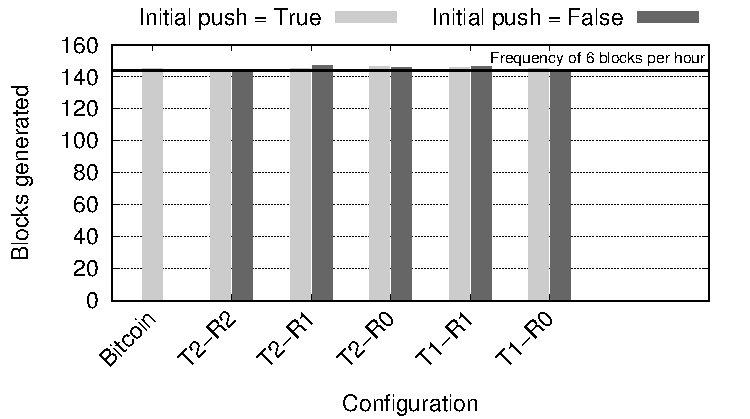
\includegraphics[width=0.5\textwidth]{plots/blocks-gen.pdf}
\caption{Blocks generated.}
\label{fig:nb-blocks}
\end{figure}

\begin{figure}
\centering
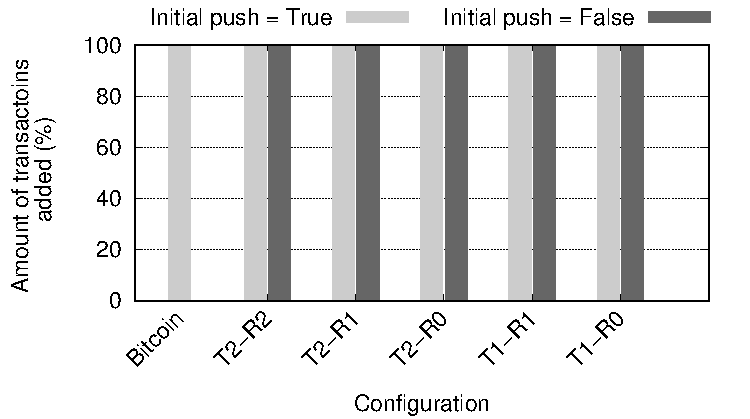
\includegraphics[width=0.5\textwidth]{plots/tx-added.pdf}
\caption{Percentage of transactions committed.}
\label{fig:tx-added}
\end{figure}

\begin{figure}
\centering
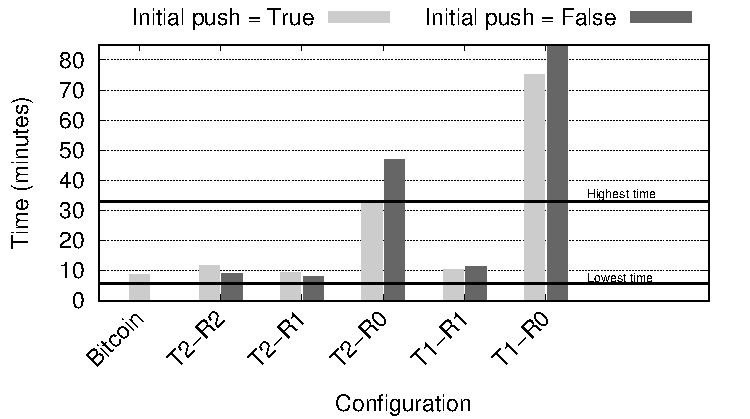
\includegraphics[width=0.5\textwidth]{plots/commit-time.pdf}
\caption{Average time it takes for a transaction to be committed.}
\label{fig:commit-time}
\end{figure}

\begin{figure}
\centering
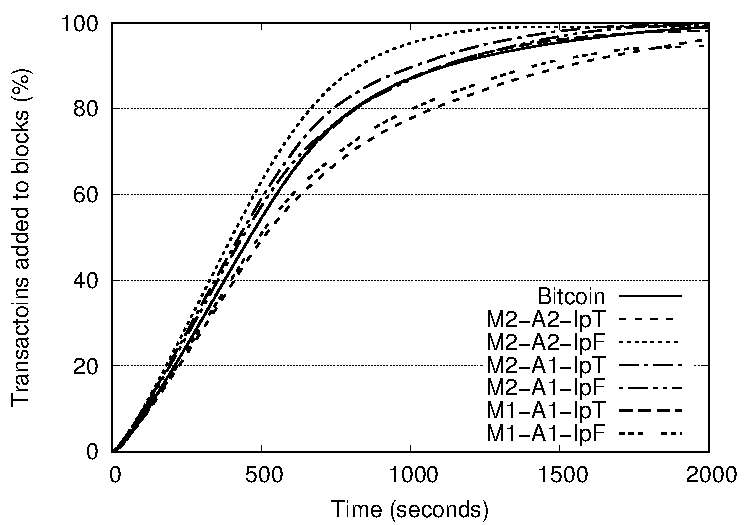
\includegraphics[width=0.5\textwidth]{plots/cdf_commit.pdf}
\caption{Cumulative function of the time it takes for a transaction to be committed.}
\label{fig:cdf-commit}
\end{figure}

\begin{figure}
\centering
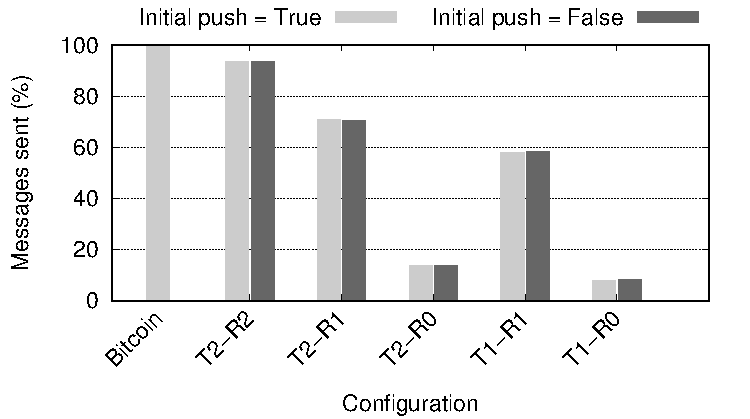
\includegraphics[width=0.5\textwidth]{plots/msg-sent.pdf}
\caption{Total number of messages sent.}
\label{fig:msg-sent}
\end{figure}

\begin{figure}
\centering
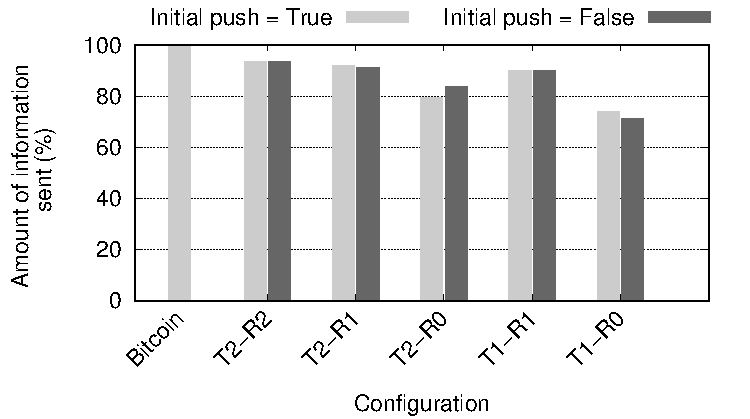
\includegraphics[width=0.5\textwidth]{plots/mb-sent.pdf}
\caption{Amount of information sent.}
\label{fig:mb-sent}
\end{figure}

\section{Conclusions}
This paragraph will end the body of this sample document.
Remember that you might still have Acknowledgments or
Appendices; brief samples of these
follow.  There is still the Bibliography to deal with; and
we will make a disclaimer about that here: with the exception
of the reference to the \LaTeX\ book, the citations in
this paper are to articles which have nothing to
do with the present subject and are used as
examples only.
%\end{document}  % This is where a 'short' article might terminate

%ACKNOWLEDGMENTS are optional
\section{Acknowledgments}
This section is optional; it is a location for you
to acknowledge grants, funding, editing assistance and
what have you.  In the present case, for example, the
authors would like to thank Gerald Murray of ACM for
his help in codifying this \textit{Author's Guide}
and the \textbf{.cls} and \textbf{.tex} files that it describes.

%
% The following two commands are all you need in the
% initial runs of your .tex file to
% produce the bibliography for the citations in your paper.
\bibliographystyle{abbrv}
\bibliography{sigproc}  % sigproc.bib is the name of the Bibliography in this case
% You must have a proper ".bib" file
%  and remember to run:
% latex bibtex latex latex
% to resolve all references
%
% ACM needs 'a single self-contained file'!
%
\end{document}
